\chapter{Contribution}\label{sec:contribution}

This thesis shall be understood as an extension to the works of Evermann et al. \cite{evermann2016} and Schönig et al. \cite{schoenig2018}, both of which were presented in the previous section. The two works have demonstrated the applicability of LSTM neural networks in Predictive Process Monitoring, but have left out the general perspective on the sequence prediction problem. Furthermore, the impact of added features to the training data was not investigated.\\

The thesis introduces said general perspective through the adaption of the approach of Shibata et al. \cite{shibata2016bipartite}. Their bipartite network architecture as well as the engineered SP-2 features have shown extraordinary performance in the SPiCE competition \cite{web:spice}. This transfer is made under the hypothesis that a case can exhibit properties similar to grammatical rules. Sub-sequence information as proposed by Klinkmüller et al. \cite{klinkmuller2018reliablemonitoring} are considered as an alternative to the SP-2 features. These sub-sequences are mined with PrefixSpan \cite{pei2001prefixspan}.

The two implementations are henceforth referred to as SP2 for the bipartite architecture using SP-2 features and PFS for the bipartite architecture using sub-sequence information mined with PrefixSpan. They are compared to the performance of implementations that mimic Evermann et al. and Schönig et al. Where original numbers were published, these are used additionally. The BPIC2011 \cite{BPIC2011} and BPIC2012 \cite{BPIC2012} datasets are used and pre-processed differently as per each approach.\\

Finally, a statement about the importance of individual features for predictions shall be made to assert whether the added overhead for feature engineering and network construction is justified by a boost in performance and prediction stability.

\section{Contrasting compared approaches}
A further contribution to current research of this thesis is the comparison of differently designed networks that solve the same prediction problem.

% Use this to plot subfigures:
% https://texblog.org/2011/05/24/placing-figures-side-by-side-subfig/

\begin{figure}[ht]
\centering
\subfloat[][]{
    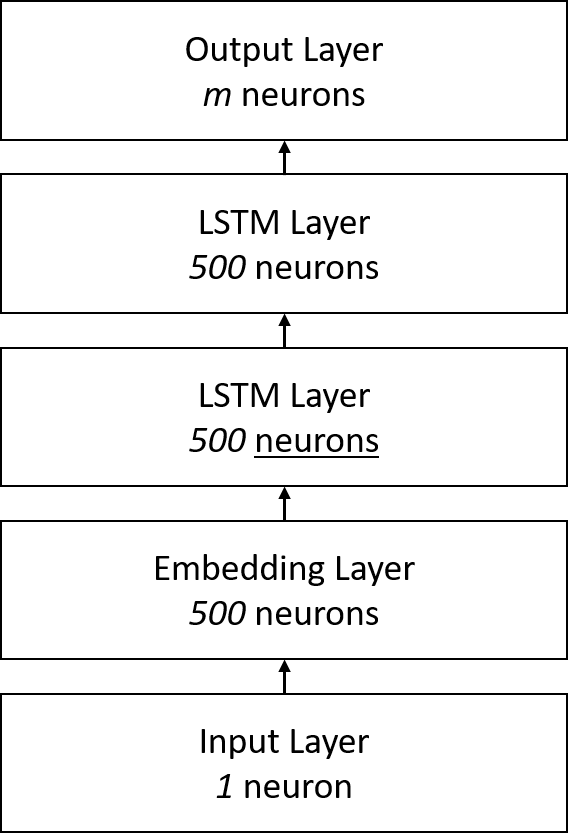
\includegraphics[width=0.4\textwidth]{gfx/evermann-network-architecture.png}
}
\qquad
\subfloat[][]{
    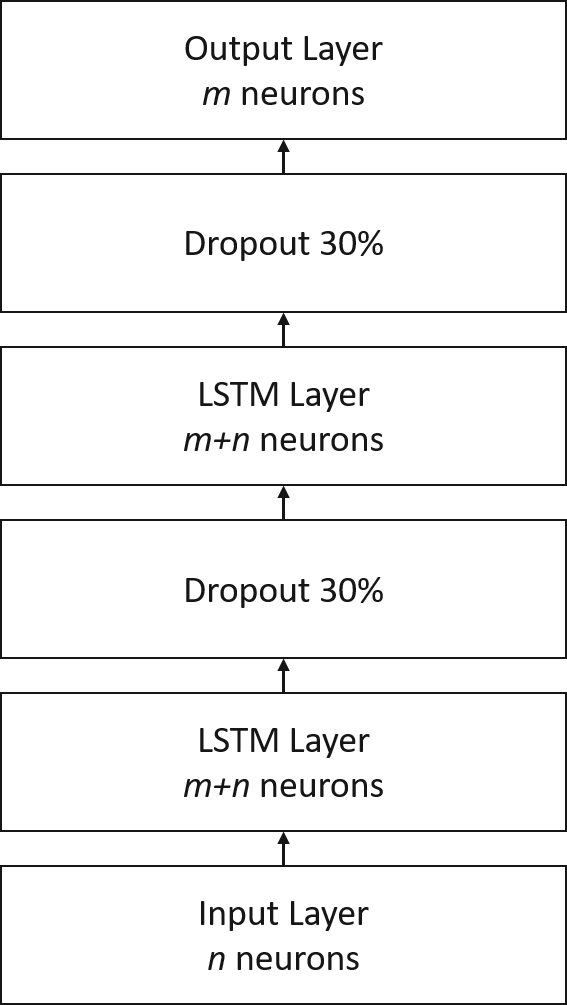
\includegraphics[width=0.4\textwidth]{gfx/schoenig-network-architecture.png}
}
\qquad
\subfloat[][]{
    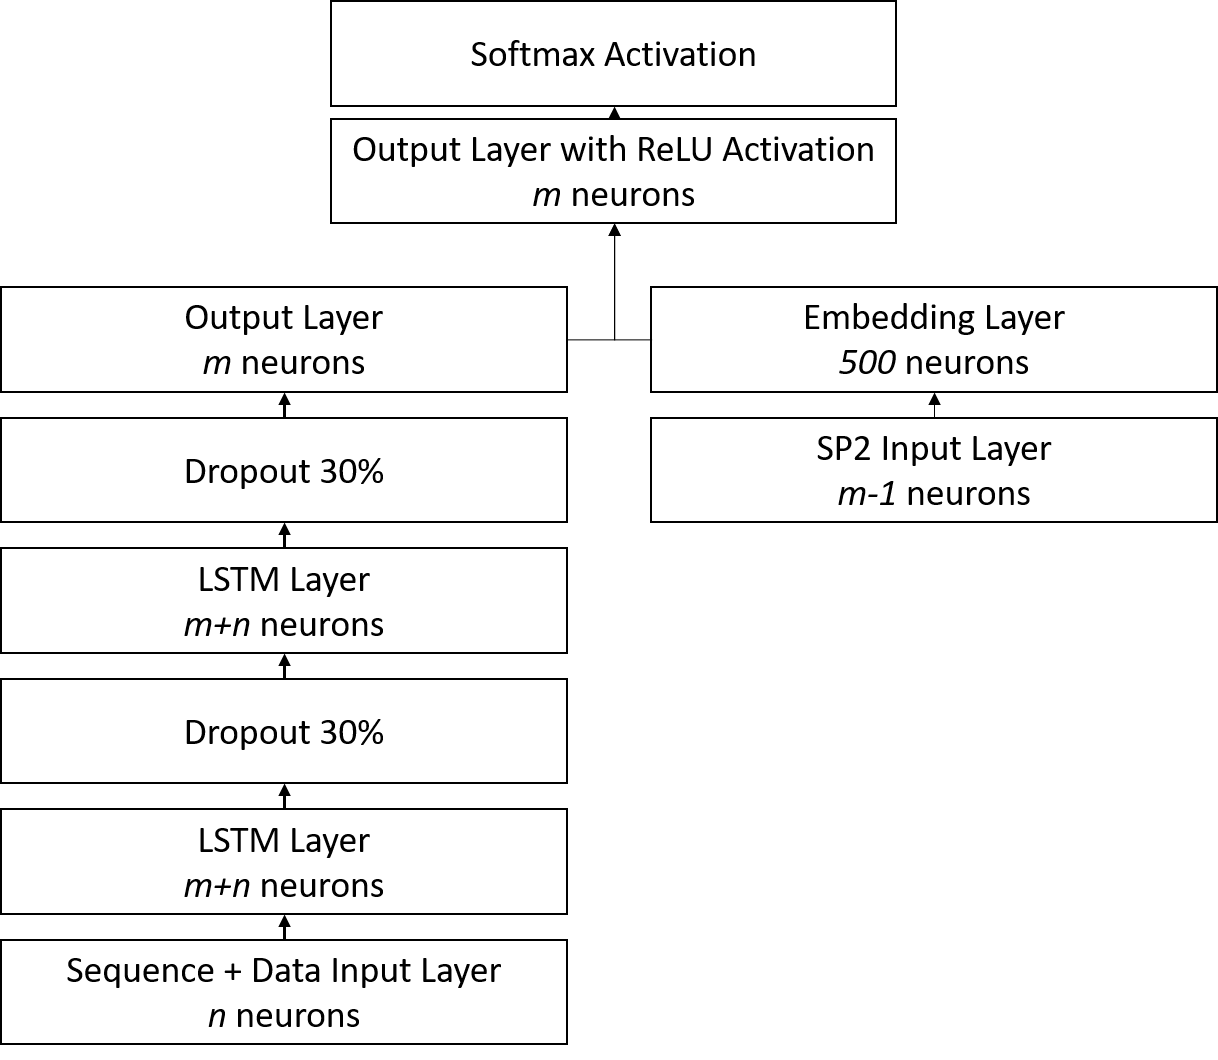
\includegraphics[width=0.4\textwidth]{gfx/sp2-network-architecture.png}
}
\qquad
\subfloat[][]{
    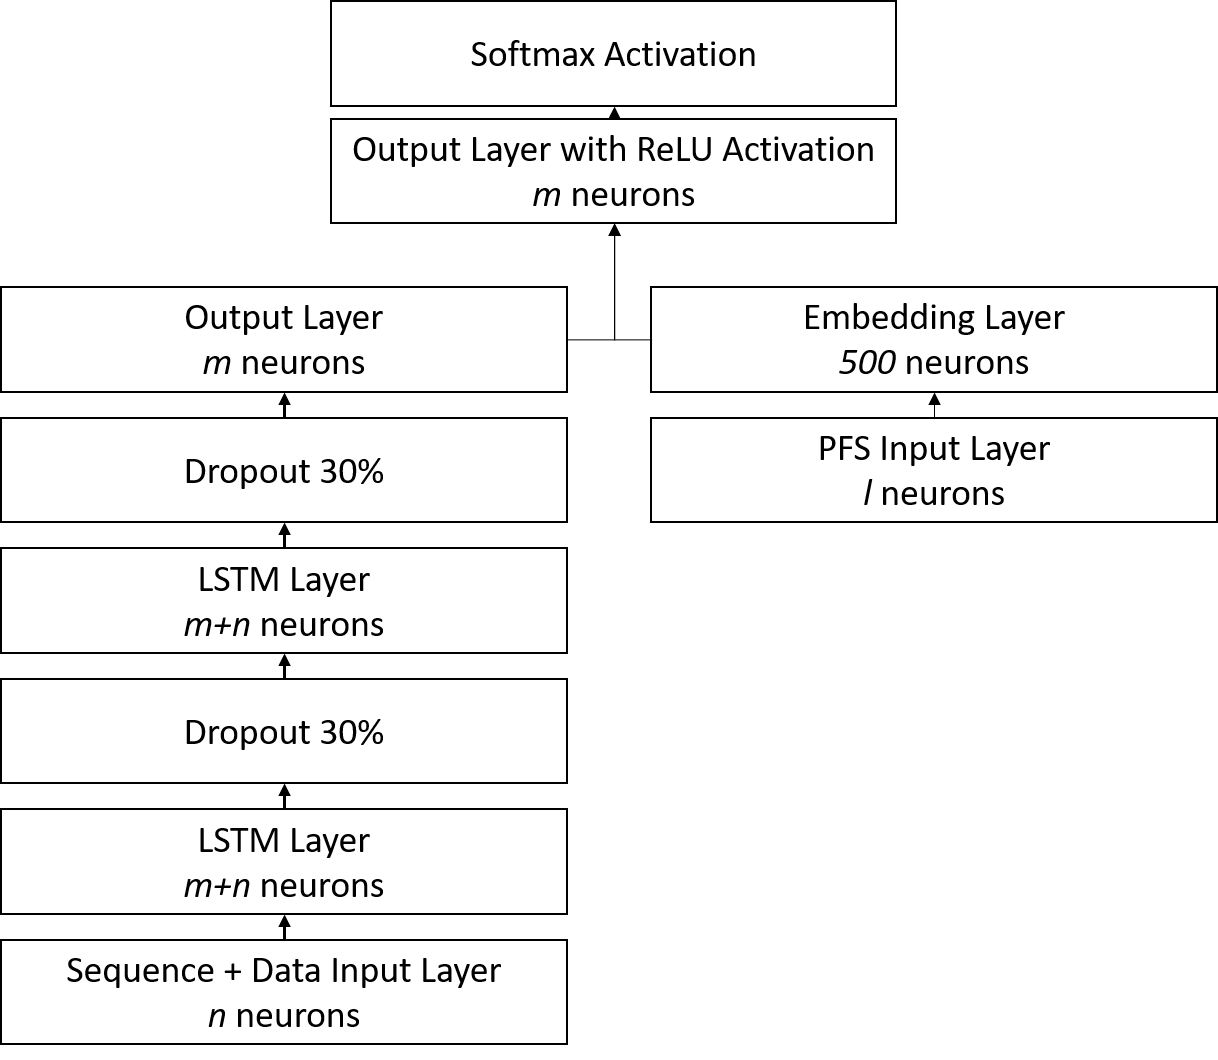
\includegraphics[width=0.4\textwidth]{gfx/pfs-network-architecture.png}
}
\caption{This is a table containing several subtables.}
\end{figure}



\section{Understanding a trace as a sequence}
Transfer an XES log to a sequence